
\chapter{Hash Tables}

\section{Direct-Address Table}
Direct addressing is a simple and efficient method when the universe \( U \) of possible keys is relatively small. A direct-address table \( T \) is an array where:
\[
T[i] = \text{value associated with key } i
\]
Given \( U = \{0, 1, \dots, m-1\} \), \( T \) is of size \( m \).

\subsection{Operations}
\begin{figure}[H]
    \centering
    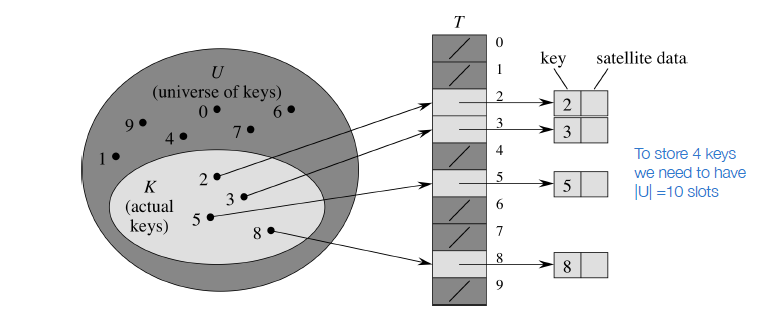
\includegraphics[width=0.75\linewidth]{direct-adress table.png}
    \label{fig:enter-label}
\end{figure}

\begin{itemize}
    \item \texttt{Direct-Table-Search(T, k):} Returns \( T[k] \), \( O(1) \).
    \item \texttt{Direct-Table-Insert(T, x):} Returns \( T[x.key] = x \), \( O(1) \).
    \item \texttt{Direct-Table-Delete(T, x):} Returns \( T[x.key] = NIL \), \( O(1) \).
\end{itemize}



While the first is a time-efficient approach, the 2nd and 3rd approaches becomes space-inefficient if \( |U| \gg |K| \), where \( K \) is the actual set of keys.

\section{Hash Tables}
Hash tables address the inefficiency of direct addressing by using a hash function \( h: U \to \{0, 1, \dots, m-1\} \), which maps keys to slots of a fixed-size table \( T[0,1,...,m-1] \). $\\$



\title{Hash Tables Overview}

\begin{itemize}
    \item Hash tables use a table size proportional to \( |K| \), losing the direct address ability.
    \item Direct-addressing maps \( k \to T[k] \), but wastes space if \( U \) (key space) is large.
    \item A \textbf{hash function} \( h \) maps keys to table slots:
    \[
    h : U \to \{ 0, 1, \dots, m-1 \}
    \]
    \item Keys are placed in \( T[h(k)] \) instead of \( T[k] \), optimizing storage.
\end{itemize}




\subsection{Hash Function}
A hash function should:
\begin{itemize}
    \item Be simple and fast to compute.
    \item Avoid collisions.
    \item Distribute keys evenly among cells.
\end{itemize}
Example: Let \( h(k) = k \mod 6 \), \( T[0..5] \):
\begin{itemize}
    \item Insert 7: \( 7 \mod 6 = 1 \)
    \item Insert 18: \( 18 \mod 6 = 0 \)
    \item Insert 41: \( 41 \mod 6 = 5 \)
    \item Insert 34: \( 34 \mod 6 = 4 \)
    \item Insert 10: \( 10 \mod 6 = 4 \) (collision with \( 34 \)).
\end{itemize}

\begin{figure}[H]
    \centering
    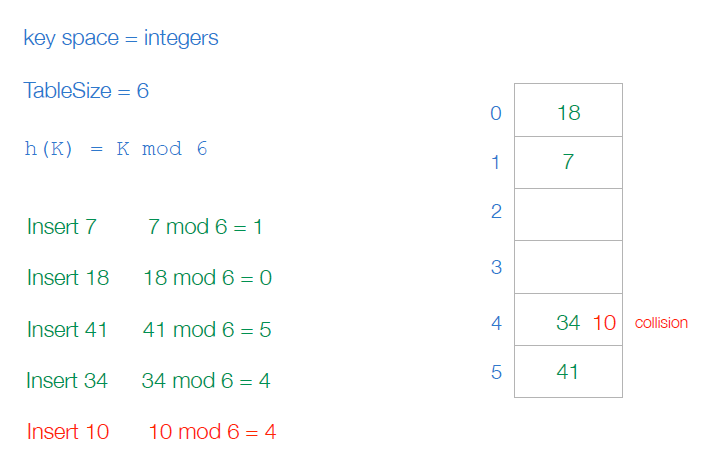
\includegraphics[width=0.75\linewidth]{hash function exam.png}
    \label{fig:enter-label}
\end{figure}


\section{Collision Resolution Strategies}

\subsection{Separate Chaining}
Collisions are resolved by maintaining a linked list at each slot.
\begin{itemize}
    \item \texttt{Insert:} \( O(1) \) if the element is unique, otherwise \( O(1 + \text{SEARCH}) \).
    \item \texttt{Search:} Proportional to the list length at the slot.
    \item \texttt{Delete:} \( O(1 + \text{SEARCH}) \).
\end{itemize}
Performance depends on the \textbf{load factor} \( \alpha = \frac{n}{m} \), where \( n \) is the number of elements and \( m \) is the size of the table. $\\$
The load factor is the average number of elements stored in a hash table where \(\alpha \in[0,1]\). Therefore the worst case is $\Theta (n)$.

\begin{figure}[H]
    \centering
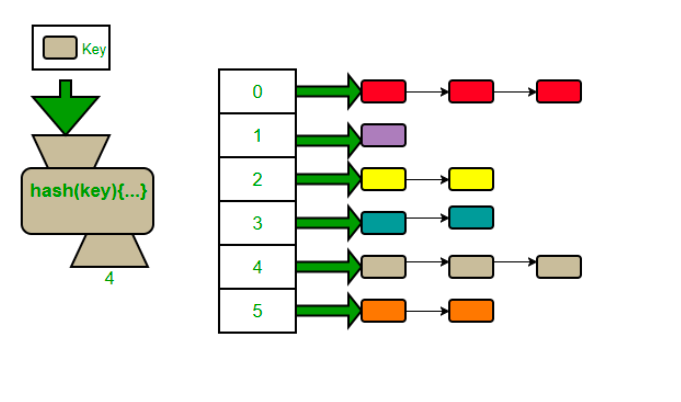
\includegraphics[width=0.75\linewidth]{separe chaining.png}
\end{figure}



\section{Simple Uniform Hashing}

\begin{itemize}
    \item For \( j = 0, 1, \dots, m-1 \), let \( T[j] \) denote the list corresponding to slot \( j \) with length \( n_j \), such that:
    \[
    n = n_0 + n_1 + \dots + n_{m-1}.
    \]
    \item The expected value of \( n_j \) is:
    \[
    \mathbb{E}[n_j] = \alpha = \frac{n}{m},
    \]
    where \( \alpha \) is the load factor.
    \item The average running time for a successful search in a hash table using chaining and assuming simple uniform hashing is:
    \[
    \Theta(1 + \alpha).
    \]
    \item If \( m \) is proportional to \( n \), then \( n = O(m) \) and:
    \[
    \alpha = \frac{n}{m} = \frac{O(m)}{m} = O(1).
    \]
\end{itemize}



\subsection*{Division Method}
The hash function is defined as:
\[
h(k) = k \mod m
\]
where \( k \) is the key, and \( m \) is the table size. 
\begin{itemize}
    \item Choose \( m \) as a prime number not close to a power of 2.
    \item Example: For \( n = 2000 \) keys and 3 collisions per list, estimate \( m \approx 666 \). A good choice is \( m = 701 \).
\end{itemize}

\subsection{Alternative Methods}
\begin{itemize}
    \item \textbf{Multiplication Method}:
    \[
    h(k) = \lfloor m \cdot (kA \mod 1) \rfloor
    \]
    where \( A \approx 0.61803 \) (Knuth's suggestion).
   \item \textbf{Squaring Method}:
    \begin{itemize}
        \item Square the key and extract middle bits.
        \item Often use \( m = 2^p \) for simpler computation.
    \end{itemize}

\end{itemize}







\subsection{Open Addressing}
Instead of linked lists (which requires the implementation of a second data structure), all data is stored directly in the table (we need a bigger table and the load factor should be below 0.5). When a collision occurs, alternative cells are probed until an empty slot is found.
Strategies include:
\begin{enumerate}
    \item \textbf{Linear Probing:} \( h_i(k) = (h(k) + i) \mod m \).
    \item \textbf{Quadratic Probing:} \( h_i(k) = (h(k) + i^2) \mod m \).
    \item \textbf{Double Hashing:} \( h_i(k) = (h(k) + i \cdot g(k)) \mod m \), where \( g \) is a second hash function.
\end{enumerate}

\subsubsection{Linear Probing Example}

\textbf{Probe Sequence:}  
When resolving collisions using linear probing, the probe sequence is defined as follows:

\begin{itemize}
    \item \( 0^\text{th} \) probe: \( h(k) = k \mod \text{TableSize} \),
    \item \( 1^\text{st} \) probe: \( (h(k) + 1) \mod \text{TableSize} \),
    \item \( 2^\text{nd} \) probe: \( (h(k) + 2) \mod \text{TableSize} \),
    \item \(\dots\),
    \item \( i^\text{th} \) probe: \( (h(k) + i) \mod \text{TableSize} \).
\end{itemize}
\textbf{Key Properties:}
\begin{itemize}
    \item A function of \( i \) is added to the original hash value to resolve collisions.
    \item Any key that hashes into an existing cluster:
    \begin{enumerate}
        \item Will require multiple attempts to resolve the collision.
        \item Will contribute to the cluster, increasing its size.
    \end{enumerate}
\end{itemize}


\begin{figure}[H]
    \centering
    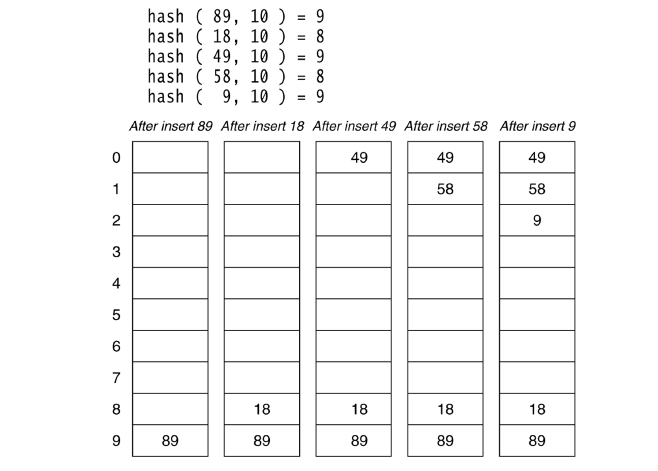
\includegraphics[width=0.75\linewidth]{linear probing.png}
\end{figure}




\subsection{Open Addressing: Search and Insertion}  

In open addressing, the search process uses the same probe sequence as insertion. For example, searching for 58 takes 4 probes, while searching for 19 takes 5.  

The average number of cells examined during insertion with linear probing is:  
\[
\frac{1 + \frac{1}{(1 - \alpha)^2}}{2}
\]  
The cost of successfully searching for an element equals the cost of its insertion.  

When the table is half full (\( \alpha = 0.5 \)), the average insertion cost is 2.5, and this remains true for future searches.  

For unsuccessful searches, the average cost is:  
\[
\frac{1 + \frac{1}{(1 - \alpha)^2}}{2}
\]  
For successful searches:  
\[
\frac{1 + \frac{1}{1 - \alpha}}{2}
\]  
At \( \alpha = 0.5 \), insertion typically examines 2.5 cells.  

Primary clustering worsens as the table fills, but when half empty, the effect is minimal.  

\subsection{Linear Probing Example:}
\begin{figure}[H]
    \centering
    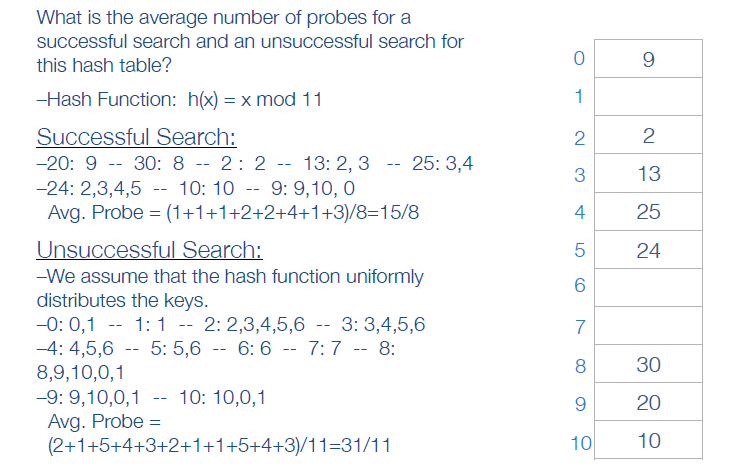
\includegraphics[width=0.75\linewidth]{LP example.png}
\end{figure}

\subsubsection{Primary Clustering}
It works pretty well for an empty table and gets worse as the table fills up.
If a bunch of elements hash to the same spot, they clash with each other. But, worse, if a bunch of elements hash to the same area of the table, they keep clashing! (Even though the hash function isn’t producing lots of collisions!)$\\$
This phenomenon is called primary clustering and Linear probing suffers from \textbf{primary clustering}, where elements form clusters that grow, increasing the likelihood of future collisions.

\begin{figure}[H]
    \centering
    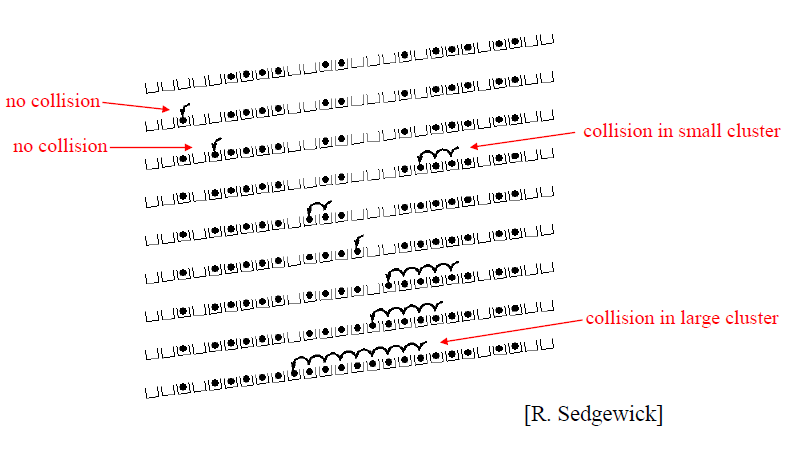
\includegraphics[width=0.75\linewidth]{primary clustering.png}
    \caption{Enter Caption}
    \label{fig:enter-label}
\end{figure}

\subsubsection{Quadratic Probing}
\textbf{Reduces Primary Clustering:} Keys that hash to nearby slots do not follow the same probe sequence.

Reduces clustering but may encounter \textbf{secondary clustering} where keys hashing to the same slot follow identical probe sequences. \( h_i(k) = (h(k) + i^2) \mod m \).

There are cases in which, due to probing, there is no available spot. If there are numbers in the same place those will cause infinite collisions. For example
\begin{align}
47 \hspace{1mm} \text{mod} \hspace{1mm} 7 =  5 \rightarrow & 5+(i^2) \\
                                               \rightarrow & 5+(i+1)^2 \\
                                               \rightarrow & 5+(i+2)^2 ...    
\end{align}
but also
\begin{align}
75 \hspace{1mm} \text{mod} \hspace{1mm} 7 =  5 \rightarrow & 5+(i^2) \\
                                               \rightarrow & 5+(i+1)^2 \\
                                               \rightarrow & 5+(i+2)^2 ...    
\end{align}
\begin{figure}[h!]
    \centering
    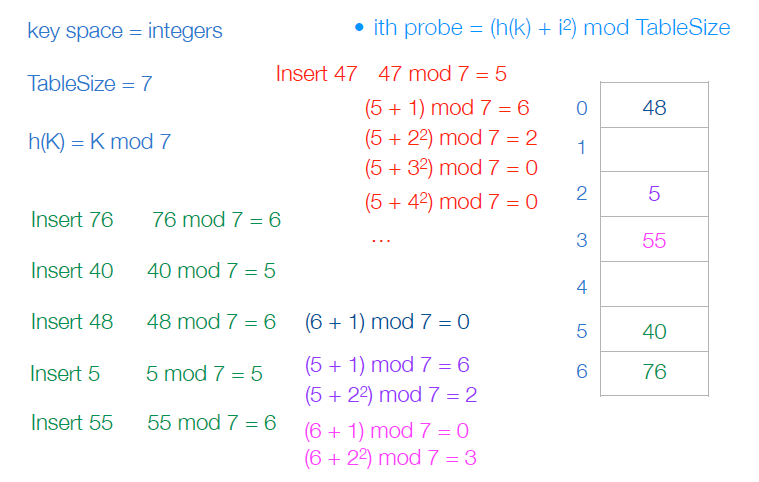
\includegraphics[width=0.75\linewidth]{quadratic probing example.png}
    \label{fig:enter-label}
\end{figure}

\subsubsection{Double Hashing Example}
Hash function \( h(k) = k \mod 7 \), \( g(k) = 5 - (k \mod 5) \):
Insert 76, 93, 40, 47, 10, 55. \newline
\textbf{Table Size:}  
 Optimal load factor \( \alpha = \frac{1}{2} \) (table twice as large as expected elements).  \newline
\textbf{Probe Calculation} Next probe:  
    \[
    (i+1)^2 - i^2 = 2i + 1
    \]
For \( \alpha < \frac{1}{2} \), an empty slot is always found. If \( \alpha > \frac{1}{2} \), a slot may not exist.  

\begin{figure}[h!]
    \centering
    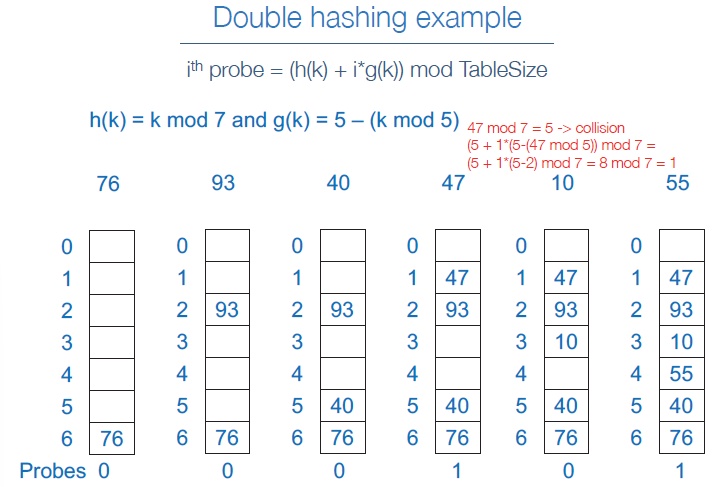
\includegraphics[width=0.75\linewidth]{immagini/doublehahing.png}
\end{figure}
\section{Rehashing}
When the table is too full (\( \alpha > 0.5 \)), rehashing is required:
\begin{itemize}
    \item Create a new table, typically twice as large.
    \item Recompute hash values for all non-deleted keys.
\end{itemize}
Rehashing costs \( O(n) \) but occurs infrequently.

\section{Python Hash Tables}
Python dictionaries are implemented as hash tables using \textbf{open addressing:}  with random probing. Collisions are handled by comparing both the hash and the key. If the hash and key match, the entry is skipped, otherwise probing continues until an empty slot is found. 
$\\$

When a new dictionary is created, it starts with 8 slots. The table resizes when it becomes two-thirds full to maintain efficiency. Each slot can store one entry, and if the slot is occupied, Python checks for a match using the == operator (not is). If no match is found, random probing selects the next slot in a pseudo-random order, continuing until the entry is placed. 
$\\$

This design ensures efficient insertion, lookup, and handling of collisions, keeping Python dictionaries fast and reliable.
